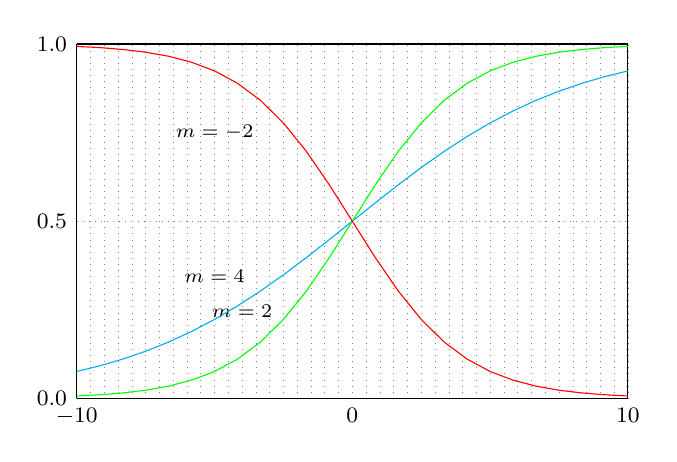
\begin{tikzpicture}[xscale=0.35,yscale=4.5]
\draw [help lines,dotted,step=0.5] (-10,0) grid (10,1);
\draw [thin] (-10,0) -- (-10,1);
\draw [thin] (-10,1) -- (10,1);
\draw [thin] (10,0) -- (10,1);
\draw [thin] (-10,0) -- (10,0);
\node [below] at (0,0) {\footnotesize{$0$}};
\node [left] at (-10,0) {\footnotesize{$0.0$}};
\node [left] at (-10,0.5) {\footnotesize{$0.5$}};
\node [left] at (-10,1) {\footnotesize{$1.0$}};
\node [below] at (-10,0) {\footnotesize{$-10$}};
\node [below] at (10,0) {\footnotesize{$10$}};
\node [below] at (-5,0.8) {\scriptsize{$m = - 2$}};
\node [above] at (-5,0.3) {\scriptsize{$m = 4$}};
\node [above] at (-4,0.2) {\scriptsize{$m = 2$}};
\draw [cyan,thin,domain=-10:10] plot (\x,{1/(1+exp(-0.25*\x))});
\draw [green,thin,domain=-10:10] plot (\x,{1/(1+exp(-0.5*\x))});
\draw [red,thin,domain=-10:10] plot (\x,{1/(1+exp(0.5*\x))});
\end{tikzpicture} 